\documentclass[11pt,a4paper]{article}
\usepackage[margin=1in]{geometry}
\usepackage[T1]{fontenc}
\usepackage[utf8]{inputenc}
\usepackage{graphicx}
\usepackage{hyperref}
\usepackage{enumitem}
\usepackage{float}
\usepackage{booktabs}

\title{Process Modeling and Process Mining\\Homework 1 — BPMN Process Modeling}
\author{Peter Dobosi}
\date{\today}

\begin{document}
\maketitle

\section{Introduction}

\subsection{Assignment}

The task for this homework is to model a (sub)system as a BPMN diagram, accompanied by a detailed written description of the processes and their mapping onto the BPMN model.
The deliverables are a textual description (this report) and an editable \texttt{.bpmn} diagram file.

\subsection{Motivation}

I am a second semester student, as such I do not have an in-progress thesis process to repurpose for this submission.
However, taking inspiration from my personal life, there is a winery business in my family which seemed like a suitable candidate to provide a process to model for this submission.
The ordering and fulfillment process seemed like a practical choice to describe and model, as it is an instance of the \textbf{Order-to-Cash (O2C)} process, covering the full lifecycle from receiving a customer order through collecting payment.

\section{Process Description}

\subsection{Participants}

While in reality the roles overlap significantly (my family members can wear many hats), for modeling purposes we define the following clean separation of concerns:

\begin{table}[H]
\centering
\begin{tabular}{@{}ll@{}}
\toprule
\textbf{Participant} & \textbf{Role} \\
\midrule
Customer          & External party who places and receives orders. Modeled as a separate pool. \\
Sales Manager     & Receives orders, records them, communicates with customers, generates invoices. \\
Warehouse Worker  & Checks stock and packaging material availability, transports wine from \\
                  & cellar if needed, procures packaging materials, packages orders. \\
Delivery Driver   & Loads the delivery van and delivers orders, collects cash payment on delivery. \\
\bottomrule
\end{tabular}
\end{table}

The three winery roles (Sales Manager, Warehouse Worker, Delivery Driver) are modeled as lanes within a single \textbf{Winery} pool.

\subsection{Process Flow}

\subsubsection{Order Receipt}

The process starts when a customer places an order. Orders can arrive through several channels: phone call, email, Facebook message, or in person (at the winery or at a festival/event).
Regardless of the channel, the Sales Manager notices and records the order details (customer name, contact information, wines requested with quantities, delivery address).

\subsubsection{Stock Availability Check}

Once the order is recorded, the Warehouse Worker first performs a \textbf{wine stock check} to determine whether all requested wine types and quantities are available:
\begin{itemize}
    \item If \textbf{partially or fully unavailable at the winery but available at the wine cellar}: the missing wine must be transported from the cellar to the winery before proceeding.
    \item If a wine type is \textbf{completely out of stock} (neither at the winery nor at the cellar): the process moves to out-of-stock handling (see below). Only once stock availability is confirmed does the process continue.
\end{itemize}

The wine stock check is performed \emph{before} the parallel split to ensure that the out-of-stock exception path (which may lead to order modification or cancellation) is fully resolved before any downstream work begins. This avoids a potential AND-join deadlock that would occur if the out-of-stock path were inside a parallel region with the packaging check.

Once wine availability is confirmed, two tasks proceed \textbf{in parallel}:
\begin{enumerate}[leftmargin=*]
    \item \textbf{Packaging material check:} The Warehouse Worker checks whether sufficient packaging materials (boxes, padding, etc.) are available. If insufficient, additional materials must be procured (purchased from a local store or ordered online). Once materials are available, the Warehouse Worker packages the order.
    \item \textbf{Invoice generation:} The Sales Manager manually generates and prints the invoice for the order.
\end{enumerate}

Both the packaging (including the packaging material check) and the invoice generation must complete before the process can proceed to delivery batching.

\subsubsection{Out-of-Stock Handling}

If any requested wine type is completely unavailable, the Sales Manager informs the customer about the unavailability. The customer can either:
\begin{itemize}
    \item \textbf{Modify the order} (substitute wines, adjust quantities) --- the process loops back to the order recording step with the updated order details.
    \item \textbf{Cancel the order} --- the process ends.
\end{itemize}

\subsubsection{Order Packaging}

The packaging of the order (placing the requested wines in the appropriate box) happens as part of the packaging material check branch of the parallel region. Once both that branch and the invoice generation branch complete, the printed invoice is included with the package and the order is ready for delivery.

\subsubsection{Delivery Batching}

Packaged orders are not delivered immediately. Instead, they are held until a delivery run is justified. A delivery run is triggered when \textbf{either}:
\begin{itemize}
    \item A single order for a delivery zone is large enough to justify the trip on its own (e.g., 6+ bottles or a high-value order), \textbf{or}
    \item Multiple smaller orders for the same delivery zone have accumulated (e.g., 3+ orders for the same area).
\end{itemize}
Until a delivery run is triggered, the packaged order waits.

\subsubsection{Loading and Delivery}

Once a delivery batch is ready, the Delivery Driver loads all orders for that delivery run into the delivery van and delivers the orders to the respective customers.

\subsubsection{Payment Collection}

Payment can occur in different ways:
\begin{itemize}
    \item \textbf{Cash on delivery} (most common): The Delivery Driver collects cash payment from the customer upon delivery.
    \item \textbf{Electronic payment} (bank transfer): The customer may pay electronically at any time up until delivery.
\end{itemize}

To handle both payment methods robustly, the Sales Manager's payment status check runs \textbf{in parallel} with the Delivery Driver's loading and delivery:
\begin{itemize}
    \item \textbf{Branch A (Sales Manager):} The Sales Manager checks whether electronic payment has been received. This check may take time, as it involves verifying bank statements or payment confirmations.
    \item \textbf{Branch B (Delivery Driver):} The Delivery Driver loads the delivery van and delivers the orders to the customers.
\end{itemize}

Both branches must complete before proceeding. Once the delivery is done and the payment status is known, a decision is made:
\begin{itemize}
    \item If electronic payment \textbf{has been received}: no further action is needed.
    \item If electronic payment \textbf{has not been received}: the Delivery Driver collects cash payment from the customer as a fallback.
\end{itemize}

This parallel structure ensures that the payment check covers the entire window up to (and including) the delivery itself, avoiding a race condition where a payment arriving after a pre-departure check but before delivery would be missed.

After payment is collected (or confirmed as already received), the order is considered fulfilled and the process ends.

\section{BPMN Model}

\subsection{BPMN Elements Used}

\begin{table}[H]
\centering
\begin{tabular}{@{}ll@{}}
\toprule
\textbf{BPMN Element} & \textbf{Usage in This Process} \\
\midrule
Pools              & Customer (external), Winery (internal) \\
Lanes              & Sales Manager, Warehouse Worker, Delivery Driver \\
Start Event        & Order received \\
End Events         & Order fulfilled, Order cancelled \\
Parallel Gateway   & Packaging material check and invoice generation run concurrently \\
                   & (after wine stock is confirmed); payment status check runs \\
                   & concurrently with loading and delivery \\
Exclusive Gateways & Stock availability, modify/cancel decision, payment method, \\
                   & delivery batch threshold \\
Loop               & Customer modifies order $\rightarrow$ returns to order recording \\
Intermediate Event & Waiting for delivery batch to accumulate \\
Message Flow       & Communication between Customer pool and Winery pool \\
\bottomrule
\end{tabular}
\end{table}

\subsection{Diagram}

\begin{figure}[H]
    \centering
    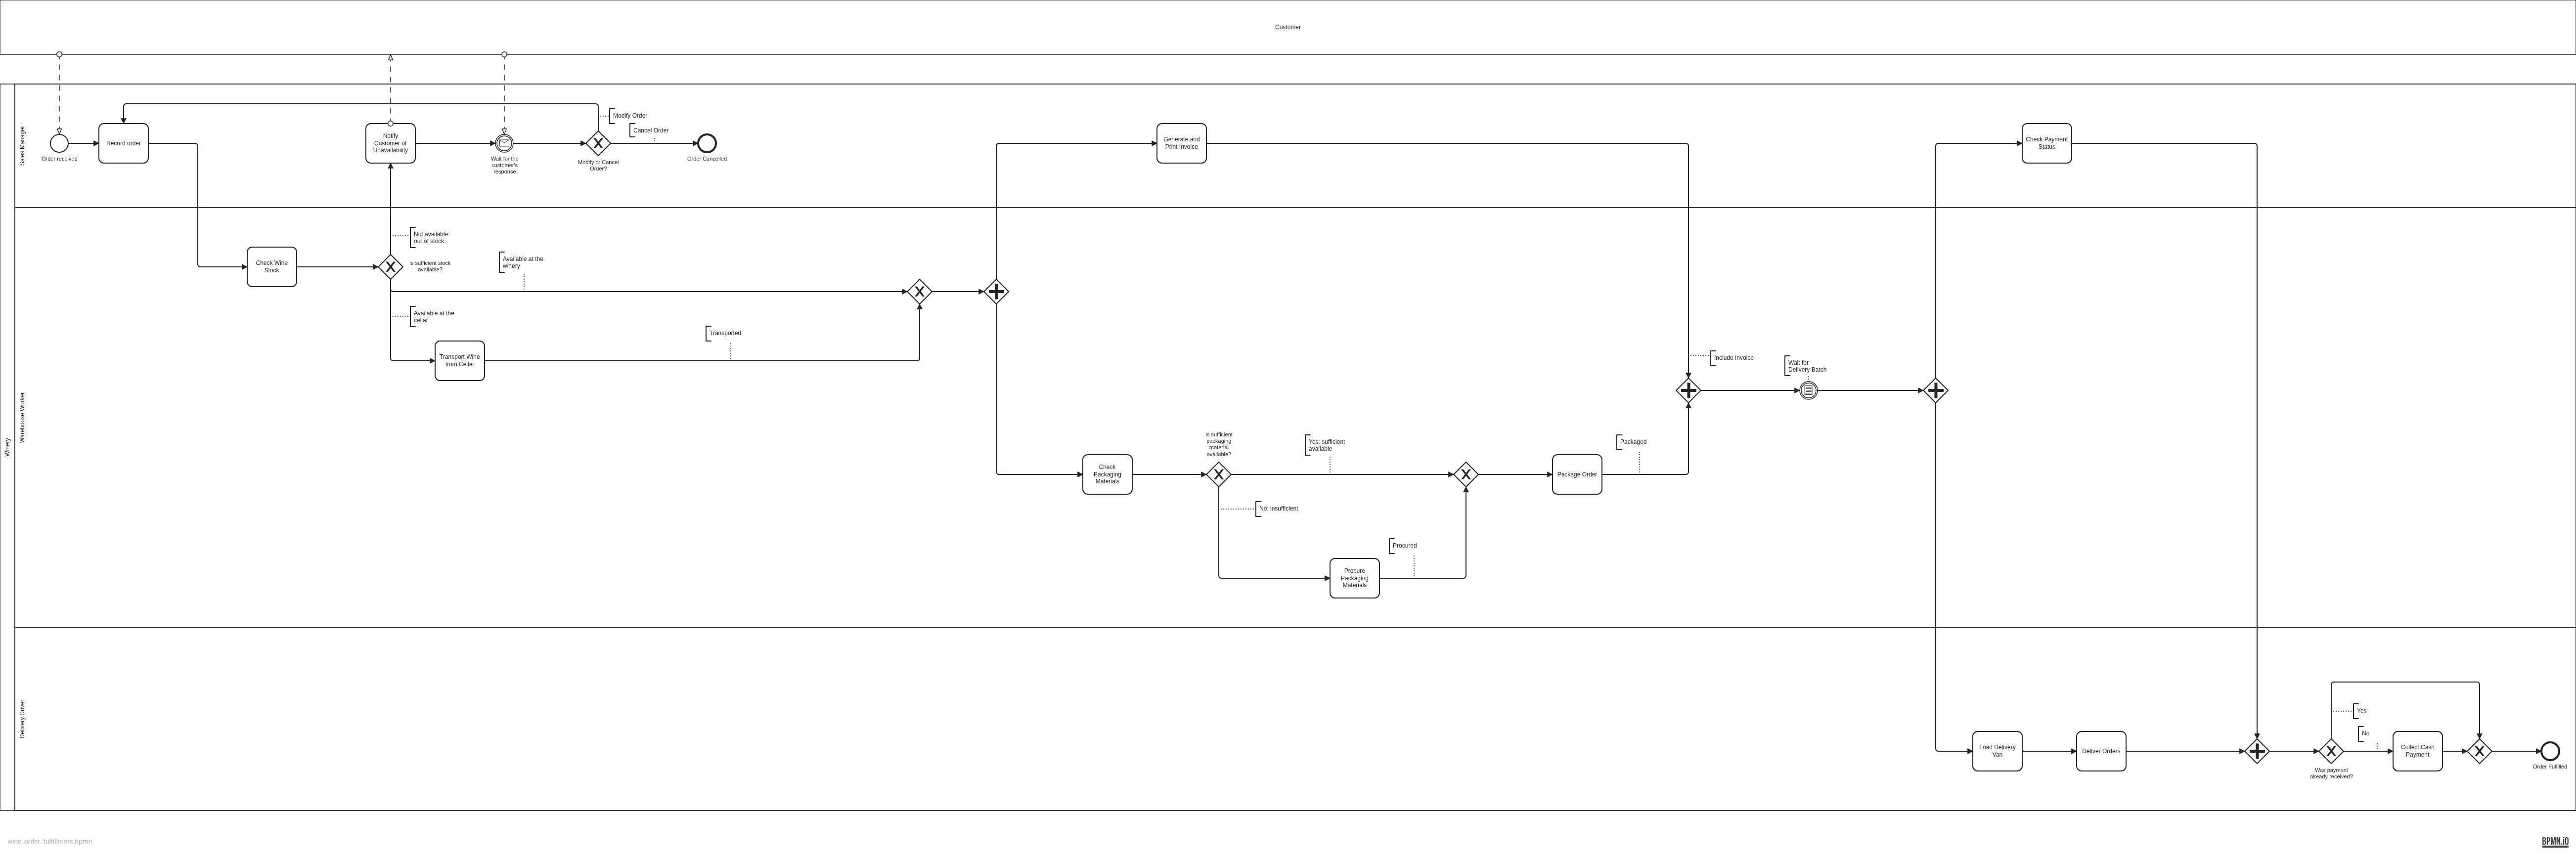
\includegraphics[width=\textwidth]{wine_order_fulfillment.png}
    \caption{BPMN model of the wine order and fulfillment process.}
    \label{fig:bpmn}
\end{figure}

\subsection{Design Decision: Sequential Wine Check}

An earlier version of this model placed the wine stock check and the packaging material check inside the same parallel region. This introduced a structural deadlock: if the wine was completely out of stock and the customer cancelled (or modified) the order, the wine branch's token would never reach the parallel join, while the packaging branch's token waited there indefinitely.

The current model resolves this by performing the wine stock check \emph{sequentially}, before the parallel split. The out-of-stock exception path (customer notification, modify/cancel decision) is therefore fully resolved before any parallel work begins. Once wine availability is confirmed, the parallel split forks into the packaging material check branch and the invoice generation branch, both of which are guaranteed to complete and converge at the downstream parallel join.

This restructuring eliminates the AND-join deadlock without requiring more complex BPMN constructs such as embedded subprocesses with boundary events or transaction scopes.

\section{Future Considerations}

The current model captures the as-is state of the winery's order-to-cash process with some idealization for modeling clarity.
Several potential improvements and extensions could be explored in a future to-be model:

\begin{enumerate}[leftmargin=*]
    \item \textbf{Batching timeout:} Currently, a packaged order waits indefinitely until the delivery threshold is met. A timer-based escalation could be introduced so that orders exceeding a maximum wait time (e.g., 5 business days) are delivered regardless of batch size, preventing customer dissatisfaction.

    \item \textbf{In-person pickup option:} Customers could be offered the option to pick up their order directly at the winery, bypassing the delivery batching and delivery steps entirely. This would introduce an additional exclusive gateway after packaging.

    \item \textbf{Ad-hoc transport via visiting guests:} If another customer or guest is traveling from the winery toward the same delivery area, orders could be sent along opportunistically, providing an alternative to the regular delivery van run.

    \item \textbf{Pre-payment upon order submission:} Instead of collecting payment only at delivery, customers could be offered (or required) to pay electronically at the time of ordering. This would shift the payment step earlier in the process and reduce the Delivery Driver's cash-handling responsibilities.

    \item \textbf{Dynamic delivery threshold calculation:} Rather than using fixed thresholds (6+ bottles or 3+ orders), the delivery trigger could be calculated dynamically based on factors such as distance to the delivery zone, fuel costs, and total order value, optimizing delivery efficiency.
\end{enumerate}

\section{Personal Notes}

This was an interesting assignment; I enjoyed working on it. I was surprised by how long it took me to complete it. The freedom provided by the task description initially deceived me into thinking that I could come up with a simple process, quickly model it, and be done with it in a couple of hours at most.

However, as I began modeling based on my initial written process description, I quickly ran into questions that, if not carefully considered, could lead to problems later in the model (e.g., when to check for payment, when to check for various stocks). All in all, with the time it took me to resolve them, I completed this assignment in roughly a day's time.

Additionally, I was surprised by the capabilities of modern agentic LLM systems:they proved to be helpful in reviewing the BPMN model, which is not something that I expected them to be capable of.

\section{Conclusion}

This report presented the order-to-cash process of a family-owned winery, from order receipt through delivery and payment collection.
The process was described textually and mapped onto a BPMN 2.0 model using pools, lanes, parallel and exclusive gateways, message flows, and loop constructs.
The model captures the key decision points (stock availability, delivery batching, payment method) and the interactions between the customer and the winery's internal roles.

\end{document}
